\subsection{Dashboard}\label{subsec:dashboard2}

The Dashboard screen is immediately after the Splash screen.
It is counted on the fact users will spend most of the time on the Dashboard screen, and so it contains the main functionalities.
This screen is divided into Top panel and Map controls.
These elements are in the higher stack layer above the map where are placed flying drones, place pins and restricted areas.
Besides, it allows displaying without wasteful \acrshort{poi}s~(\acrlong{poi})~\cite{poi}, satellite map or standard map, which contains \acrshort{poi}s, precisely like Google Maps application.

The Top panel is consists of:
\begin{itemize}
    \item \textbf{Device status} -- it contains current information about default device,
    \item \textbf{Search button} -- it opens the Search screen for searching of places, devices, aircrafts and zones,
    \item \textbf{Profile button} -- it open the Profile screen that represents the main menu of the whole application.
\end{itemize}
If a user has already logged in and planned a flight, Profile button contains a light blue circle with the number of planned flights in the top right on the circuit of that circle button.
It is able to see on the picture~\ref{fig:dashboard}.

The Map controls are consists of:
\begin{itemize}
    \item \textbf{My location button} -- it redirects to his position due to his location by \acrshort{gps} coordinates,
    \item \textbf{Map layers button} -- it is an offer allowing users to choose a map style,
    \item \textbf{Fly now button} -- this button shows drop down menu with Fly now and Plan a flight options for already logged in users, and Log in and sign up button for unauthorized users.
\end{itemize}
\newpage
These are additional elements that are shown on the Dashboard screen:
\begin{itemize}
    \item Drone detail panel, (Figure~\ref{fig:dashboard_drone_detail})
    \item Place detail panel,
    \item Zone detail panel, (Figure~\ref{fig:dashboard_zone_detail})
    \item Zone selection panel,
    \item Map layer panel.
\end{itemize}

The Drone detail panel is for showing necessary information and a flying drone and its flight parameters.
Besides, it contains the button to redirect to the full drone detail screen, where users can see all information about live flight immediately.

The Place detail panel contains necessary information about the place.
Also, if users want to plan a flight from this place, it allows them to pin this place on the map until they unpins it and Plan a flight button.
Place pinning into the map is demonstrated by a color change of the pin on the map and icon in the panel.

The Zone detail panel contains necessary information about the given zone, such as a lower altitude level, upper altitude level, name of the zone, and validation from and zone status.

The Zone selection is used to select a zone if a user clicks to a place in the map where is an intersection of more zones.
Simultaneously, when this selection is shown, the selected zones are highlighted.
If a user chooses a zone, the zone will show Zone detail panel and it will be highlighted only the particular zone instead of the intersection.

It was focused on the primary purpose of informing users about drones and restricted areas around them.
So, it was decided to keep a minimalistic design because the users needs to emphasize to important elements to them.


\begin{figure}
    \centering
    \begin{minipage}{.4\textwidth}
        \centering
        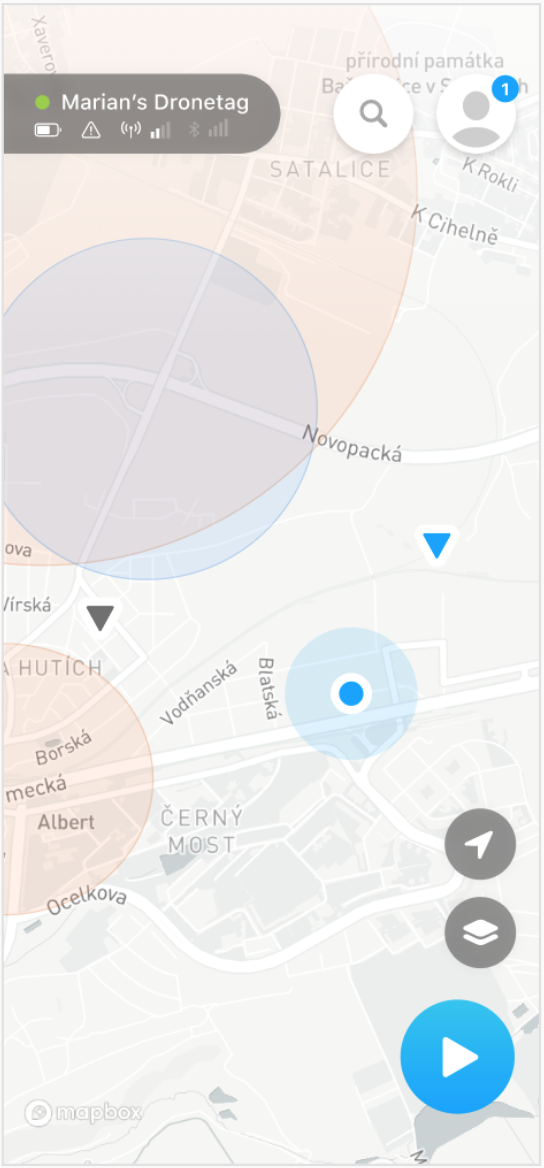
\includegraphics[width=.7\linewidth]{assets/user_interface_design/dashboard/dashboard.png}
        \caption{Dashboard}
        \label{fig:dashboard}
    \end{minipage}%
    \hspace{.05\linewidth}
    \begin{minipage}{.4\textwidth}
        \centering
        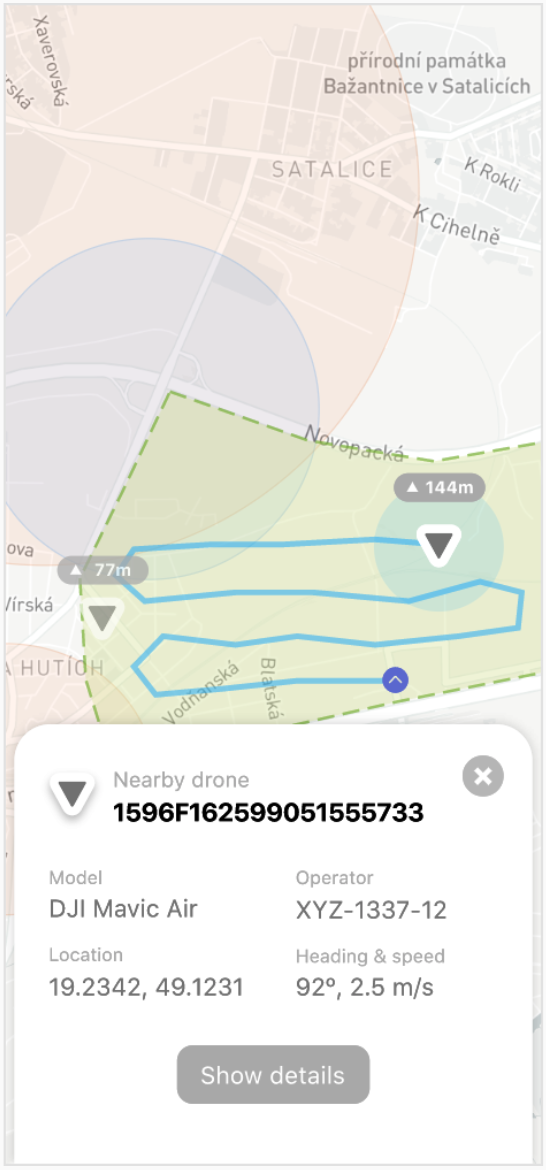
\includegraphics[width=.7\linewidth]{assets/user_interface_design/dashboard/dashboard_drone_detail.png}
        \caption{Drone detail}
        \label{fig:dashboard_drone_detail}
    \end{minipage}
    \label{fig:dashboard_all}
\end{figure}
